\documentclass{../exercisesheet}

\title{Datenkommunikation und Informationssysteme, Übung 6}
\author{
    Domenic Quirl \\ 354437
    \and
    Julian Schakib \\ 353889
    \and 
    Daniel Schleiz \\ 356092
}

\renewcommand{\Exercise}{Aufgabe}
\date{Übungsgruppe 14}

\usepackage{float}
%\usepackage{siunitx}
\usepackage{color}
\usepackage{multirow}
\usepackage{float}

\begin{document}
\maketitle
\pointtable


\begin{exercise}{4}
\begin{subexercise}
\begin{itemize}
	\item Paket 1 Header:
	\begin{description}
		\item[Version:] 4
		\item[IHL:] 5 $\hat{=}$ 20 Byte
		\item[Type of Service:] Priorität 0 = normales Datagramm, keine Flags
		\item[Total Length:] 64 Byte
		\item[Identification:] 54024
		\item[DF:] 1
		\item[MF:] 0
		\item[Offset:] 0
		\item[TTL:] 64
		\item[Protocol:] 6 = TCP
		\item[Checksum:] 7cd5
		\item[SA:] 172.16.11.12
		\item[DA:] 96.17.211.172
	\end{description}
	\item Paket 2 Header:
	\begin{description}
		\item[Version:] 4
		\item[IHL:] 5 $\hat{=}$ 20 Byte
		\item[Type of Service:] Priorität 1, keine Flags
		\item[Total Length:] 60 Byte
		\item[Identification:] 0
		\item[DF:] 1
		\item[MF:] 0
		\item[Offset:] 0
		\item[TTL:] 58
		\item[Protocol:] 6 = TCP
		\item[Checksum:] 55c2
		\item[SA:] 96.17.211.172
		\item[DA:] 172.16.11.12
	\end{description}
\end{itemize}
\begin{description}
\item[i)] \ \\
IP-Adresse meines Rechners: 172.16.11.12\\
IP-Adresse des Internetservers: 96.17.211.172
\item[ii)] \ \\
Wenn Rechner und Server dieselben Parameter verwenden, sendet der Server genau wie der Rechner mit einer TTL von 64. Wenn der Rechner vom Server also ein Paket mit TTL 58 empfängt und jeder Router auf dem Weg die TTL um 1 verringert, ergibt sich als Anzahl von Routern $64-58=6$.
\end{description}
\end{subexercise}
\begin{subexercise}
\begin{description}
\item[i)] ::ffff:c0a8:0b2a : Die Adresse liegt in ::ffff:0:0/96, dem Subnetz von IPv6, welches den IPv4-Adressbereich integriert. Sie entspricht der IPv4-Adresse 192.168.11.42.
\item[ii)] 2b0f::c56e:0000::339d:bcfc : Dieser String ist keine gültige IPv6-Adresse. IPv6 erlaubt das Weglassen von Nuller-Blöcken nur an einer Stelle, damit die Adresse eindeutig bleibt. In diesem Beispiel fehlen zum Beispiel drei Nuller-Blöcke, sodass man sowohl 2b0f:0000:c56e:0000:0000:0000:339d:bcfc als auch 2b0f:0000:0000:c56e:0000:0000:339d:bcfc konstruieren könnte.
\item[iii)] ff00:bab1:0039:9c0b::e6ce:6629 : Ist im Gegensatz zu (ii) gültig. Da die Adresse mit ff00 beginnt, liegt sie im Subnetz der Multicast-Adressen ff00::/8, ist aber keine Broadcast-Adresse.
\end{description}
\end{subexercise}
\begin{subexercise}
Das Entfernen der Prüfsumme bietet den großen Vorteil, dass diese nicht von jedem Router neu berechnet werden muss, weil dieser die TTL dekrementiert.

Dass der Wegfall nicht zu großen Problemen führt, liegt zum einen daran, dass der IPv6 Header, obwohl insgesamt aufgrund der längeren Adressen länger, aufgeräumter ist als der IPv4 Header. Es ist also weniger wahrscheinlich, dass Kontrollinformationen verfälscht werden, wenn ein Fehler auftritt, trifft er am ehesten eine der Adressen, was dann dazu führt, dass entweder das aktuelle Paket oder eine Antwort nicht ankommt und daher auf einer höheren Schicht im Zweifelsfall erneut gesendet wird. Außerdem implementieren viele Protokolle der Sicherungsschicht ihrerseits bereits eine Prüfsumme (z.B. CRC) für die gesendeten Daten.
\end{subexercise}
\end{exercise}


\begin{exercise}{6}
\begin{subexercise}
Es werden Bezeichnungen wie TL für Total Length gemäß Folie IV-50 genutzt.\\
	Router 1 sendet 3 Fragmente:
	\begin{itemize}
	\item TL=1228 ID=42 MF=1 Offset=0
	\item TL=1228 ID=42 MF=1 Offset=151
	\item TL=404 ID=42 MF=0 Offset=302
	\end{itemize}
	Von Router 2 zum Empfänger müssen die ersten beiden Fragmente nochmal fragmentiert werden, da diese die MTU überschreiten. Insgesamt sendet Router 2 also folgende
	5 Fragmente:
	\begin{itemize}
	\item TL=660 ID=42 MF=1 Offset=0
	\item TL=588 ID=42 MF=1 Offset=80
	\item TL=660 ID=42 MF=1 Offset=151
	\item TL=588 ID=42 MF=1 Offset=231
	\item TL=404 ID=42 MF=0 Offset=302
	\end{itemize}
\end{subexercise}
\begin{subexercise}
Unter der Annahme, dass die ID's bei 0 beginnen, existieren also $2^{16}$ verschiedene ID's. Falls innerhalb von einer Sekunde mehr als $2^{16}$ Pakete verschickt werden, ist das erste
noch nicht angekommen und es wird eine ID doppelt verteilt. Die Datenrate darf somit nur maximal $\frac{2^{16} \cdot 1500 \text{ Byte}}{1\text{s}}= 
98304000 \text{ Byte/s}= 98,304 \text{ MByte/s}$ betragen.
\end{subexercise}
\begin{subexercise}
Dies ist nicht problematisch, da in den IP-Headern der Fragmente neben der ID noch ebenfalls die Destination Address steht, wodurch die Empfänger trotzdem eindeutig die Fragmente
wieder zusammenbauen können.
% Ich evrstehe irgendwie die Frage nichr: Soll ein Paket, welches für z.B. Empfänger 1 bestimmt war, bei Empfänger 2 ankommen, mit gleicher ID wie das eigentlich für 2 bestimmte Paket?
\end{subexercise}
\begin{subexercise}
Ein Vorteil besteht darin, dass Zwischenstationen bei einer Übertragung entlastet werden, da die MTU für einen Pfad nur einmal berechnet werden muss und danach gecached wird, 
wodurch die Zwischenstationen im Allgemeinen weniger fragmentieren müssen. Damit lassen sich eventuell höhere Datenraten erzielen.\\
Ein Nachteil sind eventuell verloren gehende Pakete aufgrund von z.B. Firewalls: Falls beim Lernprozess der Path MTU Discovery an einer Stelle die MTU überschritten wird, aber
die darauf folgende ICMP-Meldung an den Sender durch eine Firewall abgefangen wird, denkt der Sender, das Paket sei angekommen, obwohl es verworfen wurde.
\end{subexercise}
\end{exercise}


\begin{exercise}{5}
\begin{subexercise}
\begin{figure}[H]
  \centering
  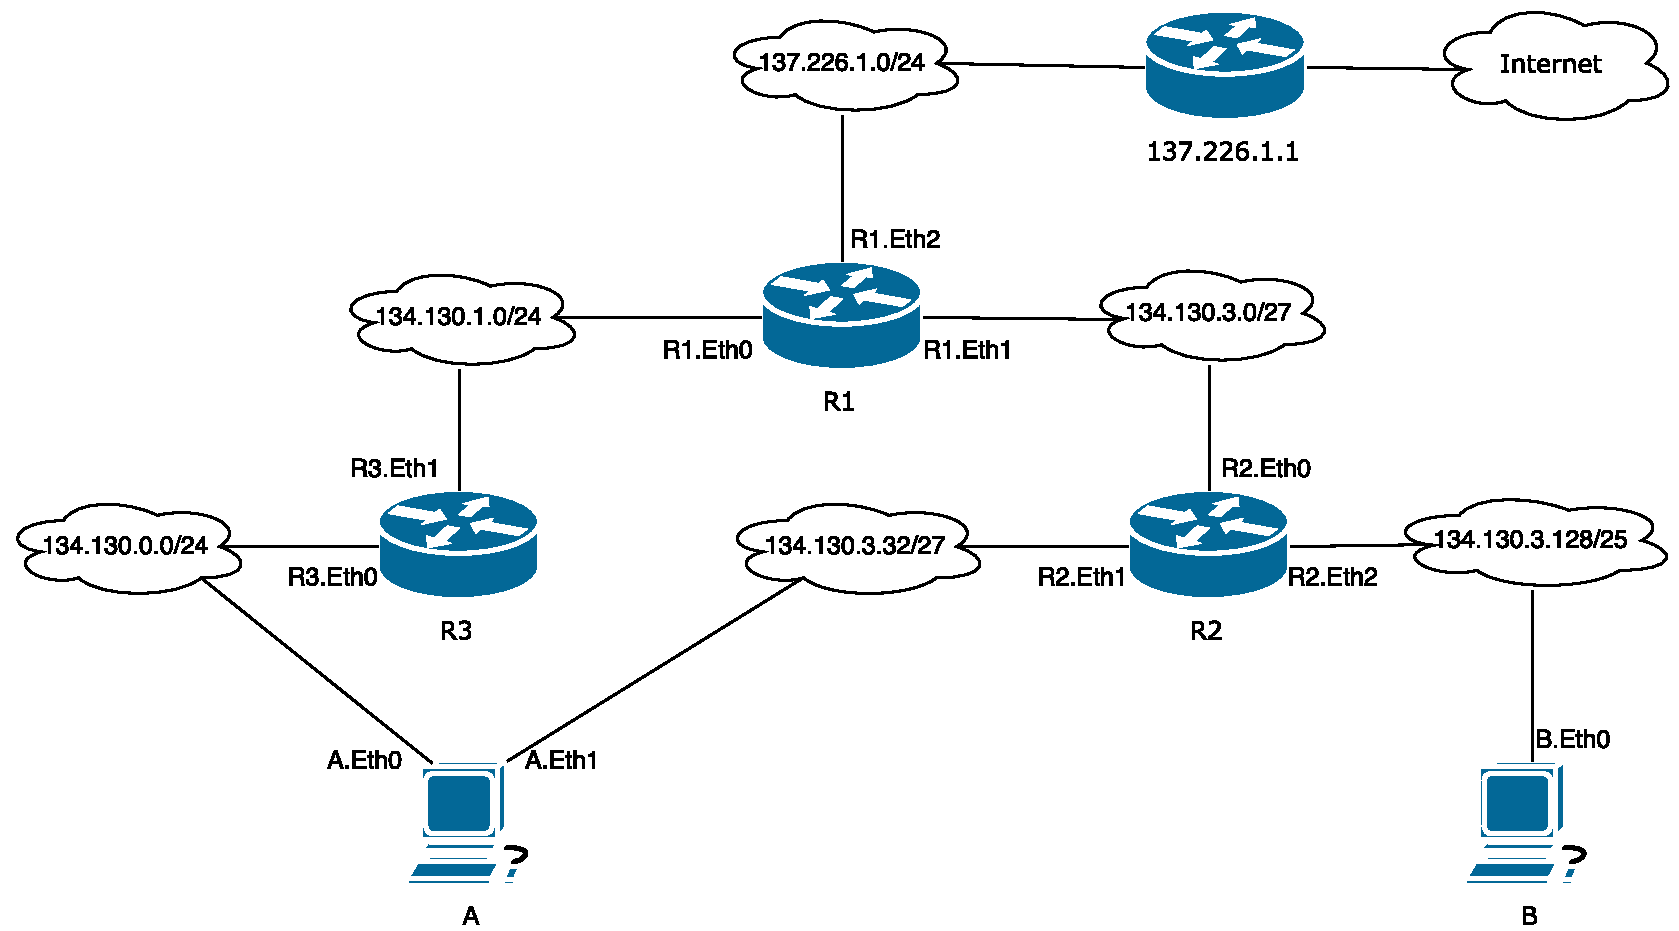
\includegraphics[width=\textwidth]{a3_network.pdf}
\end{figure}
\end{subexercise}
\begin{subexercise}
Der längste Match der IP-Adresse von B in der Tabelle von A besteht bei \texttt{0.0.0.0/0}, somit sendet A durch ETH0.\\ \ \\
\texttt{Request A.ETH0 134.130.0.152 134.130.0.1} - A erfragt die MAC von R3\\
\texttt{Reply R3.ETH0 134.130.0.1 A.ETH0 134.130.0.152} - R3 teilt A seine MAC mit\\
\texttt{Data A.ETH0 R3.ETH0} - Das Paket wird an R3 geschickt\\
\ \\
\texttt{Request R3.ETH1 134.130.1.2 134.130.1.1} - R3 erfragt die MAC von R1\\
\texttt{Reply R1.ETH0 134.130.1.1 R3.ETH1 134.130.1.2} - R1 teilt R3 seine MAC mit\\
\texttt{Data R3.ETH0 R1.ETH0} - Das Paket wird an R1 geschickt\\
\ \\
\texttt{Request R1.ETH1 134.130.3.2 134.130.3.1} - R1 erfragt die MAC von R2\\
\texttt{Reply R2.ETH0 134.130.3.1 R1.ETH1 134.130.3.2} - R2 teilt R1 seine MAC mit\\
\texttt{Data R1.ETH1 R2.ETH0} - Das Paket wird an R2 geschickt\\
\ \\
\texttt{Request R2.ETH2 134.130.3.129 134.130.3.166} - R2 erfragt die MAC von B\\
\texttt{Reply B.ETH0 134.130.3.166 R2.ETH2 134.130.3.129} - B teilt R2 seine MAC mit\\
\texttt{Data R2.ETH2 B.ETH0} - Das Paket wird an B geschickt\\
\end{subexercise}
\end{exercise}


\end{document}

